\chapter{SGSEAM Assessment Guide for Lucid BuildingOS and
BuildingDashboard}
\label{app:sgseam-lucid}

This appendix includes the SGSEAM assessment guide written specific for Lucid BuildingOS and BuildingDashboard, with the intension of administrating SGSEAM assessment to the Lucid Design Group's serious game framework. Although the assessment did not actually started, this guide illustrates an example for SGSEAM assessment to a similar serious game framework.

\section{Overview}

This document describes how to assess the Lucid BuildingOS and
BuildingDashboard using the Serious Game Stakeholder Experience
Assessment Method (SGSEAM). 

The goal of this assessment is to identify the major strengths and
shortcomings of the software framework using the perspectives of major
stakeholders. 

The cost of this assessment to Lucid is the requirement for various
stakeholders to be available to me for approximately one 30 minute interview. 

The benefit of this assessment is the identification of actionable
improvements to Lucid BuildingOS and BuildingDashboard.

The SGSEAM assessment method is being developed as part of my
Ph.D. research at the University of Hawaii.  The assessment of Lucid
BuildingOS and BuildingDashboard will help me to identify strengths
and weaknesses in SGSEAM.  All data about the LucidBuildingOS or
BuildingDashboard systems revealed through this assessment will be kept
confidential and will not be presented in my research findings. 

\autoref{fig:overview} outlines the steps of the process of applying SGSEAM to a framework.

\begin{table}[ht!]
  \center
  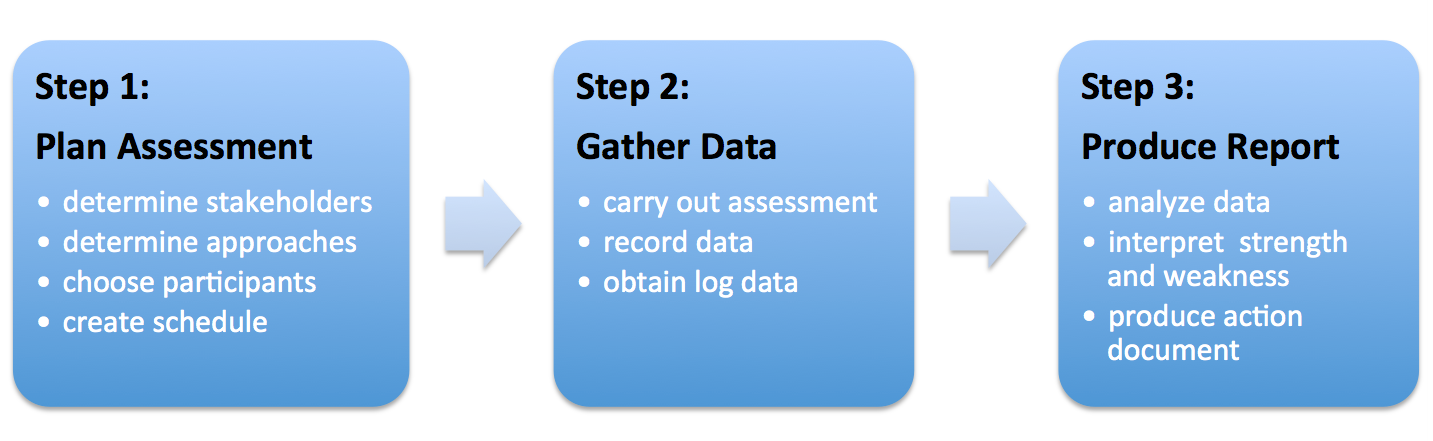
\includegraphics[width=0.8\columnwidth]{sgseam-steps}
  \caption{Applying SGSEAM to a framework}
  \label{fig:overview}
\end{table}

\begin{enumerate}
\item Step one is to plan the assessment, including
 identifying the stakeholders, determining assessment approaches, and creating the assessment schedule. 
 The deliverable for this step is the \textbf{\textit{assessment
     plan}} document. 

\item Step two is to gather data by carrying out 
 the assessment, recording and obtaining related data. The deliverable for this step is the 
 assessment \textbf{\textit{data repository}}. 

\item Step three is to produce the strength and weakness report by analyzing 
 the data and interpreting strengths and weaknesses. The deliverable
 for this step is the \textbf{\textit{improvement action}} document.

\end{enumerate}

The following chapters describe the steps in detail. The Appendix
provides additional background material. Each chapter concludes with
an ``Action Item'' shade box, which indicates what you need to do. For
example:


\begin{shadebox}
{\bf Action Item:} Read the next three chapters of this document, and determine if this proposed
evaluation is feasible. If you identify obstacles, please note them
in the spreadsheet so that we can discuss them in an upcoming phone call.
\end{shadebox}


\section{Step 1: Plan Assessment}

\subsection{Identify Stakeholders}

The first step is to identify the SGSEAM stakeholders and their tasks
for the Lucid BuildingOS and BuildingDashboard
framework. 

\begin{table}[ht!]
  \center
  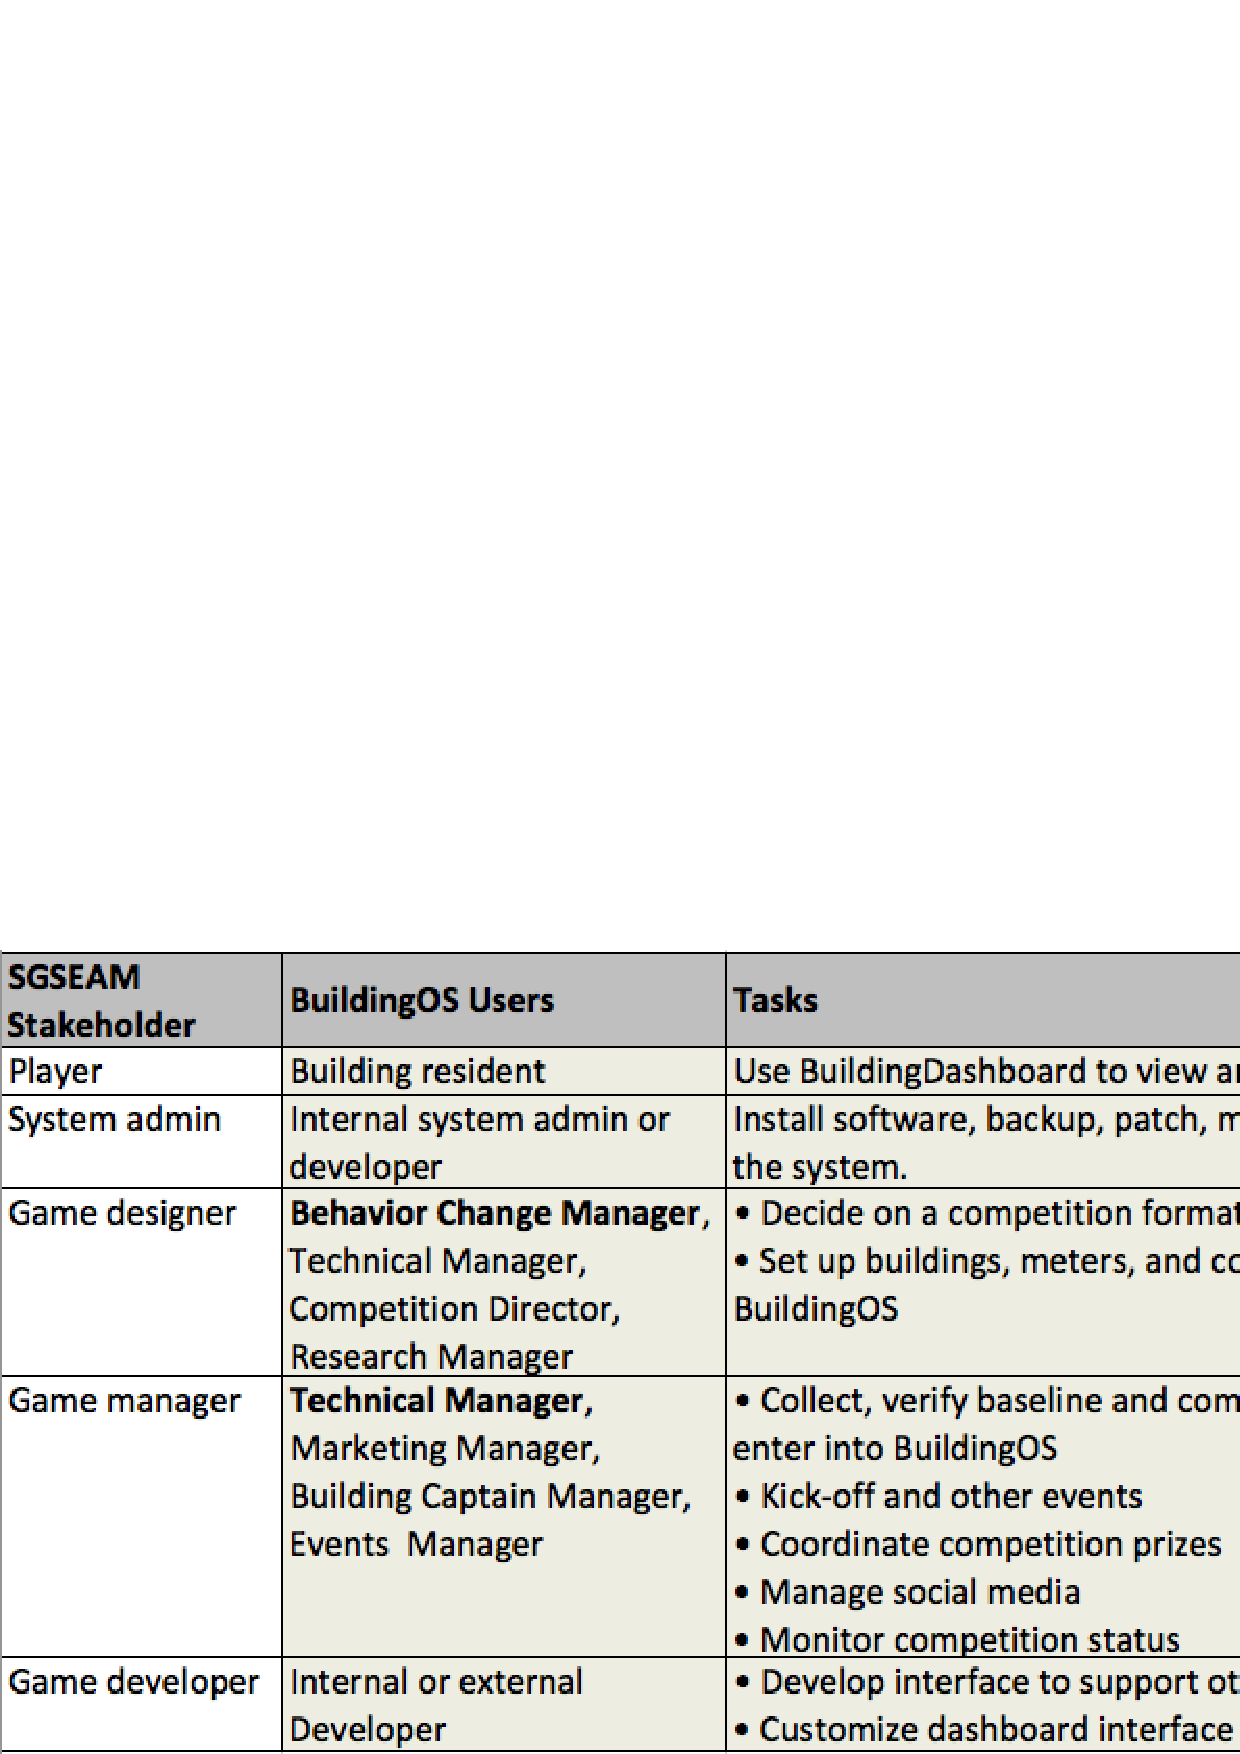
\includegraphics[width=0.9\columnwidth]{stakeholder}
  \caption{BuildingOS Stakeholders}
  \label{table:lucid-stakeholders}
\end{table}

According to Campus Conservation Nationals (CCN) Competition Planning
Guide, a Competition Organizing Team (COT) will plan and
execute the competition. Besides being residents of buildings
participating in the competition, they are also users and stakeholders
of the BuildingOS framework. 

We have converted COT roles into SGSEAM stakeholders and identified their tasks related to BuildingOS and
BuildingDashboard, as shown in
\autoref{table:lucid-stakeholders}. 

\begin{shadebox}
{\bf Action Item:} Review the ``Stakeholders'' tab in the
attached spreadsheet, and provide comments if you believe the set of
stakeholders or the mapping needs modification.
\end{shadebox}


\subsection{Determine Assessment Approach}
\label{sect:Assessment Approach}

There are several possible assessment approaches for each
stakeholder. Different assessment approaches have different levels of
rigor which impacts upon the quality the assessment
result. They also require different levels of 
implementation costs or efforts. \autoref{app:sgseam-approaches}
describes the SGSEAM assessment approaches we have developed for each
stakeholder category.

While an in-lab experiment has the most rigor, we believe it is too
expensive for this assessment. We therefore recommend an
interview approach for all stakeholders except
players. \autoref{table:lucid-approaches} shows the approaches we recommend
for each stakeholder.
 
\begin{table}[ht!]
  \center
  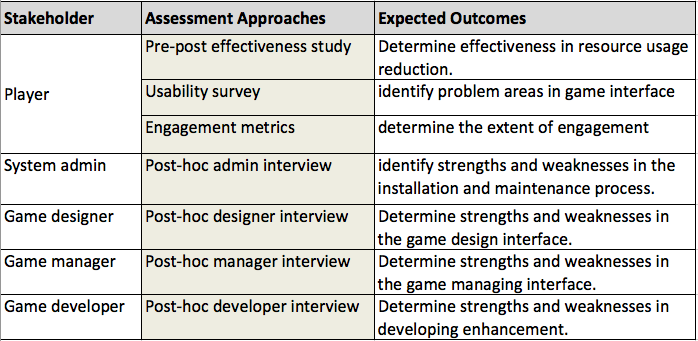
\includegraphics[width=0.9\columnwidth]{approach}
  \caption{BuildingOS Assessment Approaches}
  \label{table:lucid-approaches}
\end{table}

Refer to \autoref{app:sgseam-approaches}  for the detailed
description of the recommended approaches.

\begin{shadebox}
{\bf Action Item:} Review the ``Approach'' tab in the attached
spreadsheet.  Provide a comment if you believe an approach should be
modified, deleted, or added.
\end{shadebox}


\subsection{Choose Assessment Participants}

Once the stakeholder categories are defined, the next step is to find
individuals fitting those categories who will be willing to
participate in the evaluation process. 

\begin{table}[ht!]
  \center
  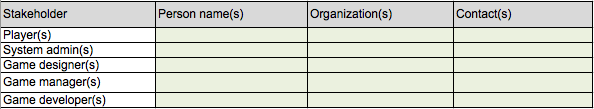
\includegraphics[width=0.9\columnwidth]{participant}
  \caption{Choose Participants}
  \label{table:participants}
\end{table}

\autoref{table:participants} shows a sample of the \textbf{\textit{Participants}} worksheet. 

For each stakeholder, identify the name(s), organization and contact
info. It is important to be able to contact the stakeholders in some
way, either via email or phone, to get the feedback from their
experiences with the framework.

\begin{shadebox}
{\bf Action Item:} Review the Participants tab in the attached
spreadsheet, and provide any individuals that you believe might be
able to participate at this point in the planning process.
\end{shadebox}

\subsection{Create Assessment Schedule}

Once we know what the assessment approaches and who the participants are, the next step is to create the assessment 
schedule. We have created a sample schedule based on the sample
planning timeline in the CCN Competition Planning Guide, as shown in
\autoref{table:schedule}. 

\begin{table}[ht!]
  \center
  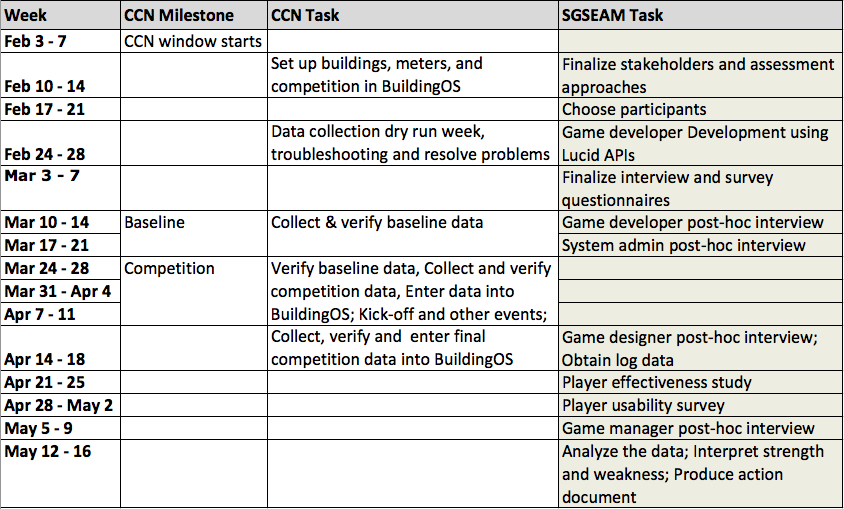
\includegraphics[width=0.9\columnwidth]{schedule}
  \caption{Assessment Schedule}
  \label{table:schedule}
\end{table}

\begin{shadebox}
{\bf Action Item:} Review the Schedule tab in the attached
spreadsheet.  Provide comments for any schedule items or dates that
you believe might need to be changed. 
\end{shadebox}

\subsection{Assess Player Stakeholder Experience}

We recommend three approaches for player assessment: pre-post effectiveness, usability survey and engagement metrics. The attached spreadsheet outlines the planned goals and survey questionnaires for these assessment approaches, as shown in \autoref{table:player}.

\begin{table}[ht!]
  \center
  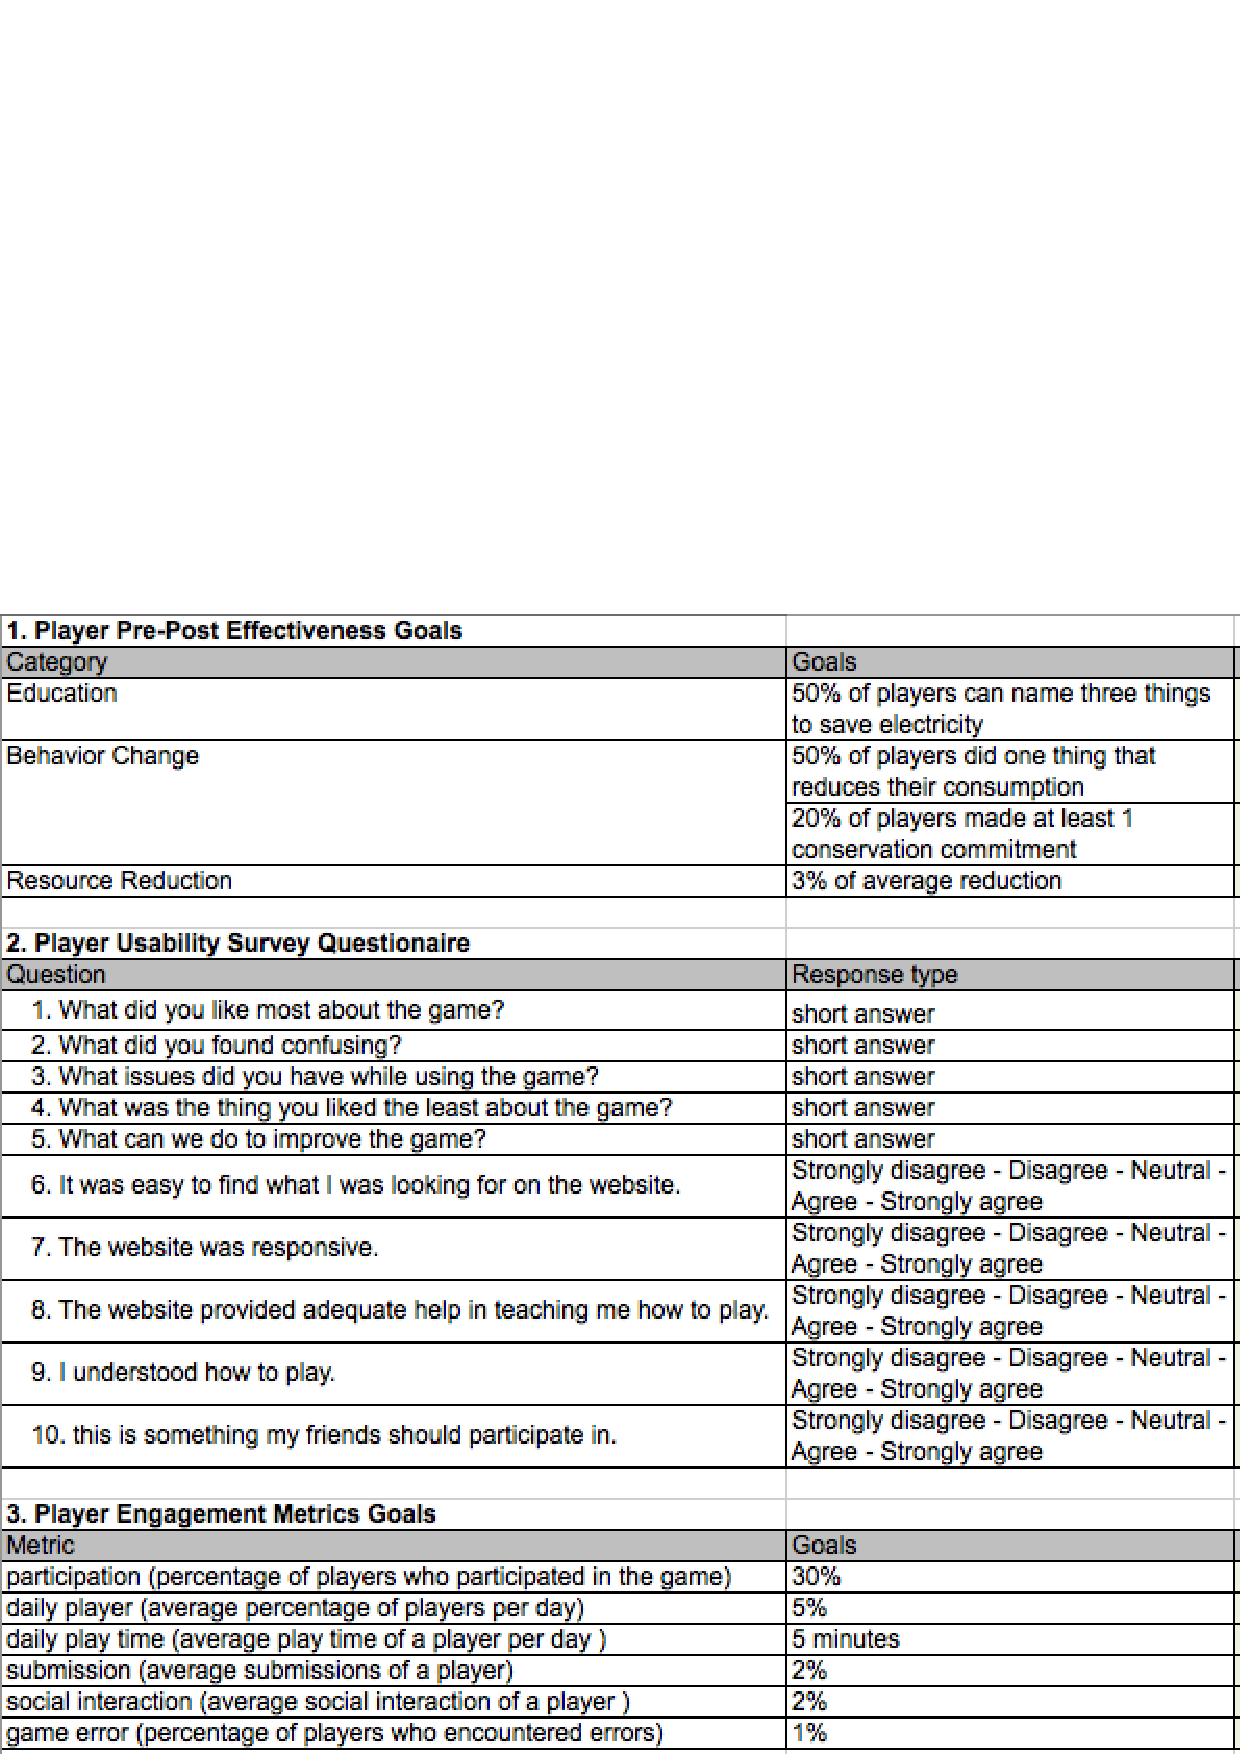
\includegraphics[width=0.9\columnwidth]{player}
  \caption{Player Assessment}
  \label{table:player}
\end{table}

\begin{shadebox}
{\bf Action Item:} Review the Player tab in the attached
spreadsheet.  Provide comments for any Player assessment items that
you believe might need to be changed. 
\end{shadebox}

\subsection{Assess System Admin Stakeholder Experience}

We recommend the post-hoc interview approach for system admin assessment. The attached spreadsheet outlines the planned interview questionnaires, as shown in \autoref{table:systemadmin}.

\begin{table}[ht!]
  \center
  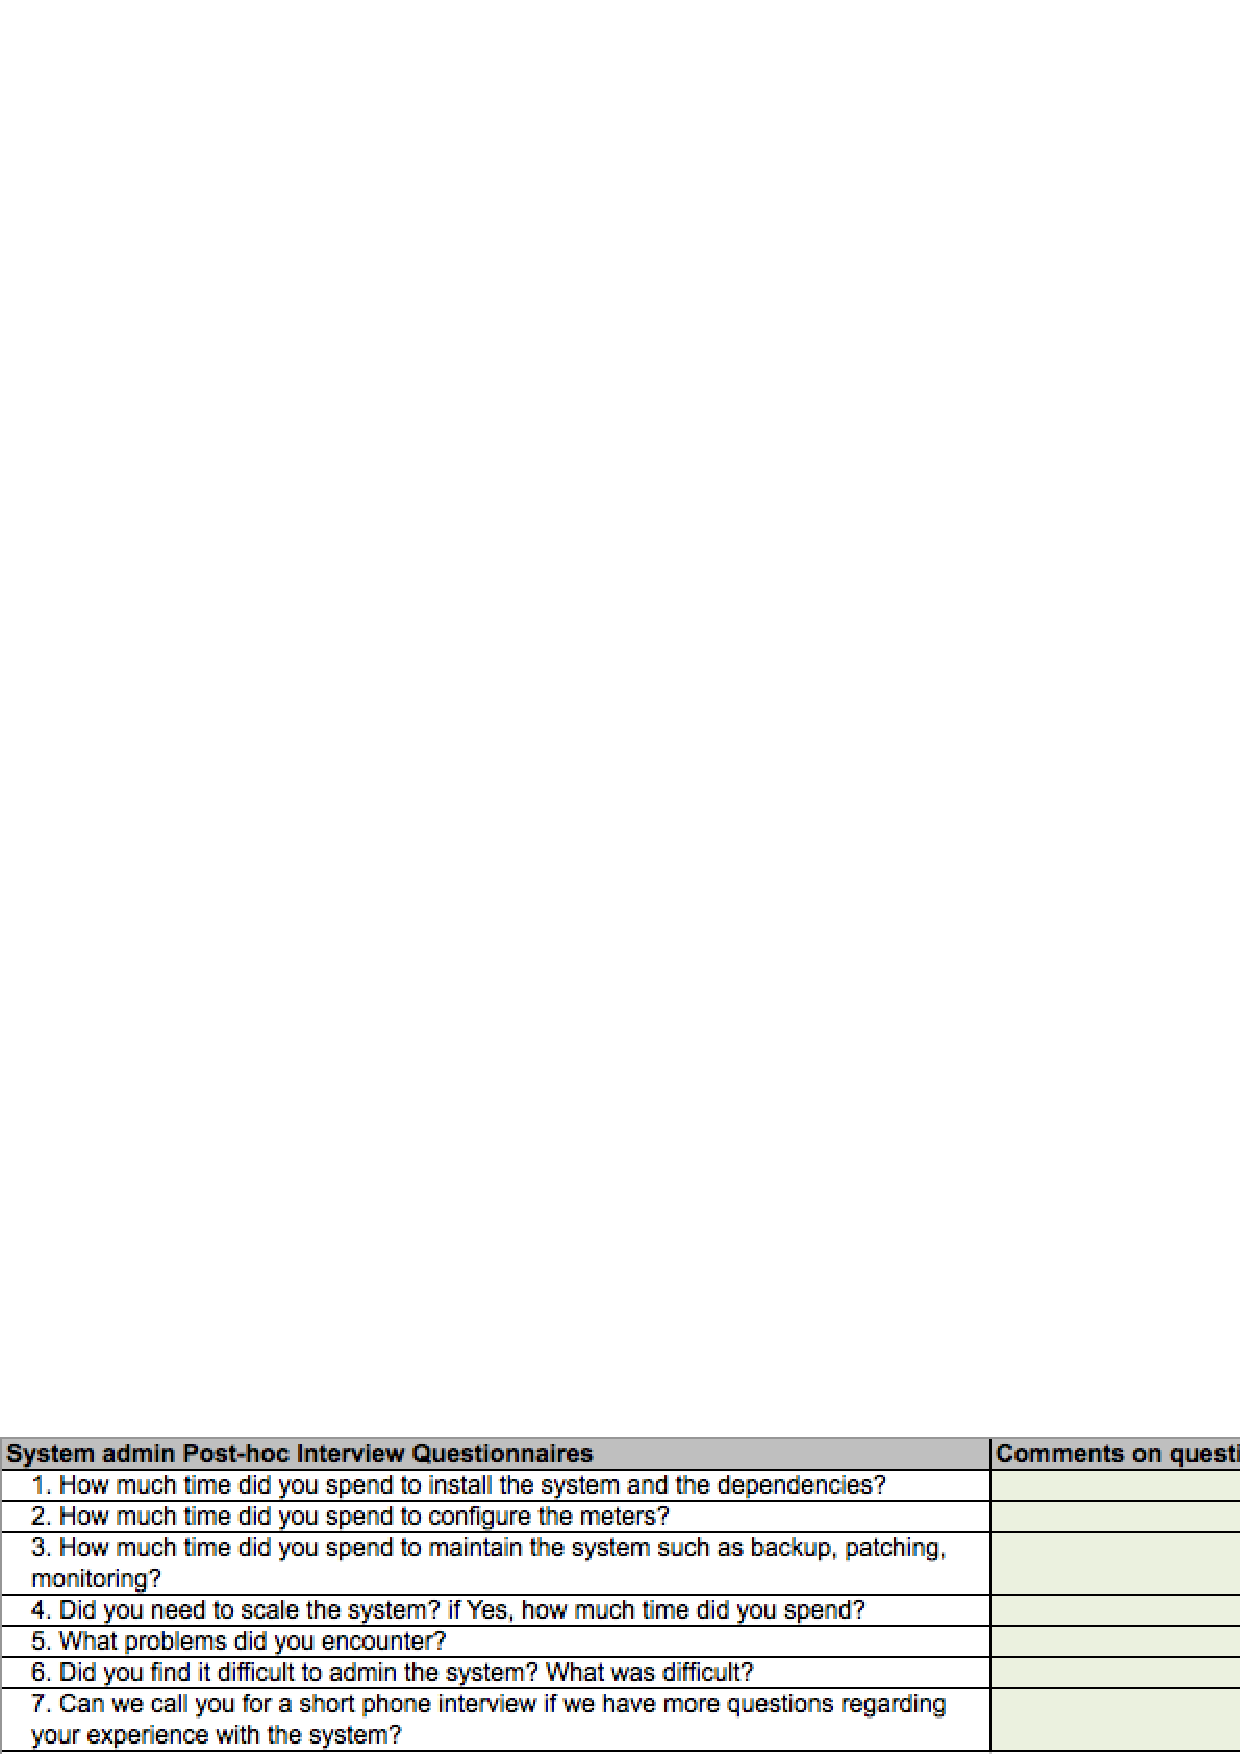
\includegraphics[width=0.9\columnwidth]{systemadmin}
  \caption{System Admin Assessment}
  \label{table:systemadmin}
\end{table}

\begin{shadebox}
{\bf Action Item:} Review the System Admin tab in the attached
spreadsheet.  Provide comments for any System Admin interview questionnaires that
you believe might need to be changed. 
\end{shadebox}

\subsection{Assess Game Designer Stakeholder Experience}

We recommend the post-hoc game designer interview approach for assessing game designer stakeholder experiences. The attached spreadsheet outlines the planned interview questionnaires for game designer, as shown in \autoref{table:designer}.

\begin{table}[ht!]
  \center
  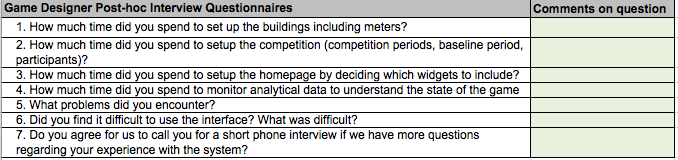
\includegraphics[width=0.9\columnwidth]{designer}
  \caption{Game Designer Assessment}
  \label{table:designer}
\end{table}

\begin{shadebox}
{\bf Action Item:} Review the Game Designer tab in the attached
spreadsheet.  Provide comments for any Game Designer interview questionnaires that
you believe might need to be changed. 
\end{shadebox}

\subsection{Assess Game Manager Stakeholder Experience}

We recommend the post-hoc interview approach for game manager assessment. The attached spreadsheet outlines the planned interview questionnaires, as shown in \autoref{table:manager}.

\begin{table}[ht!]
  \center
  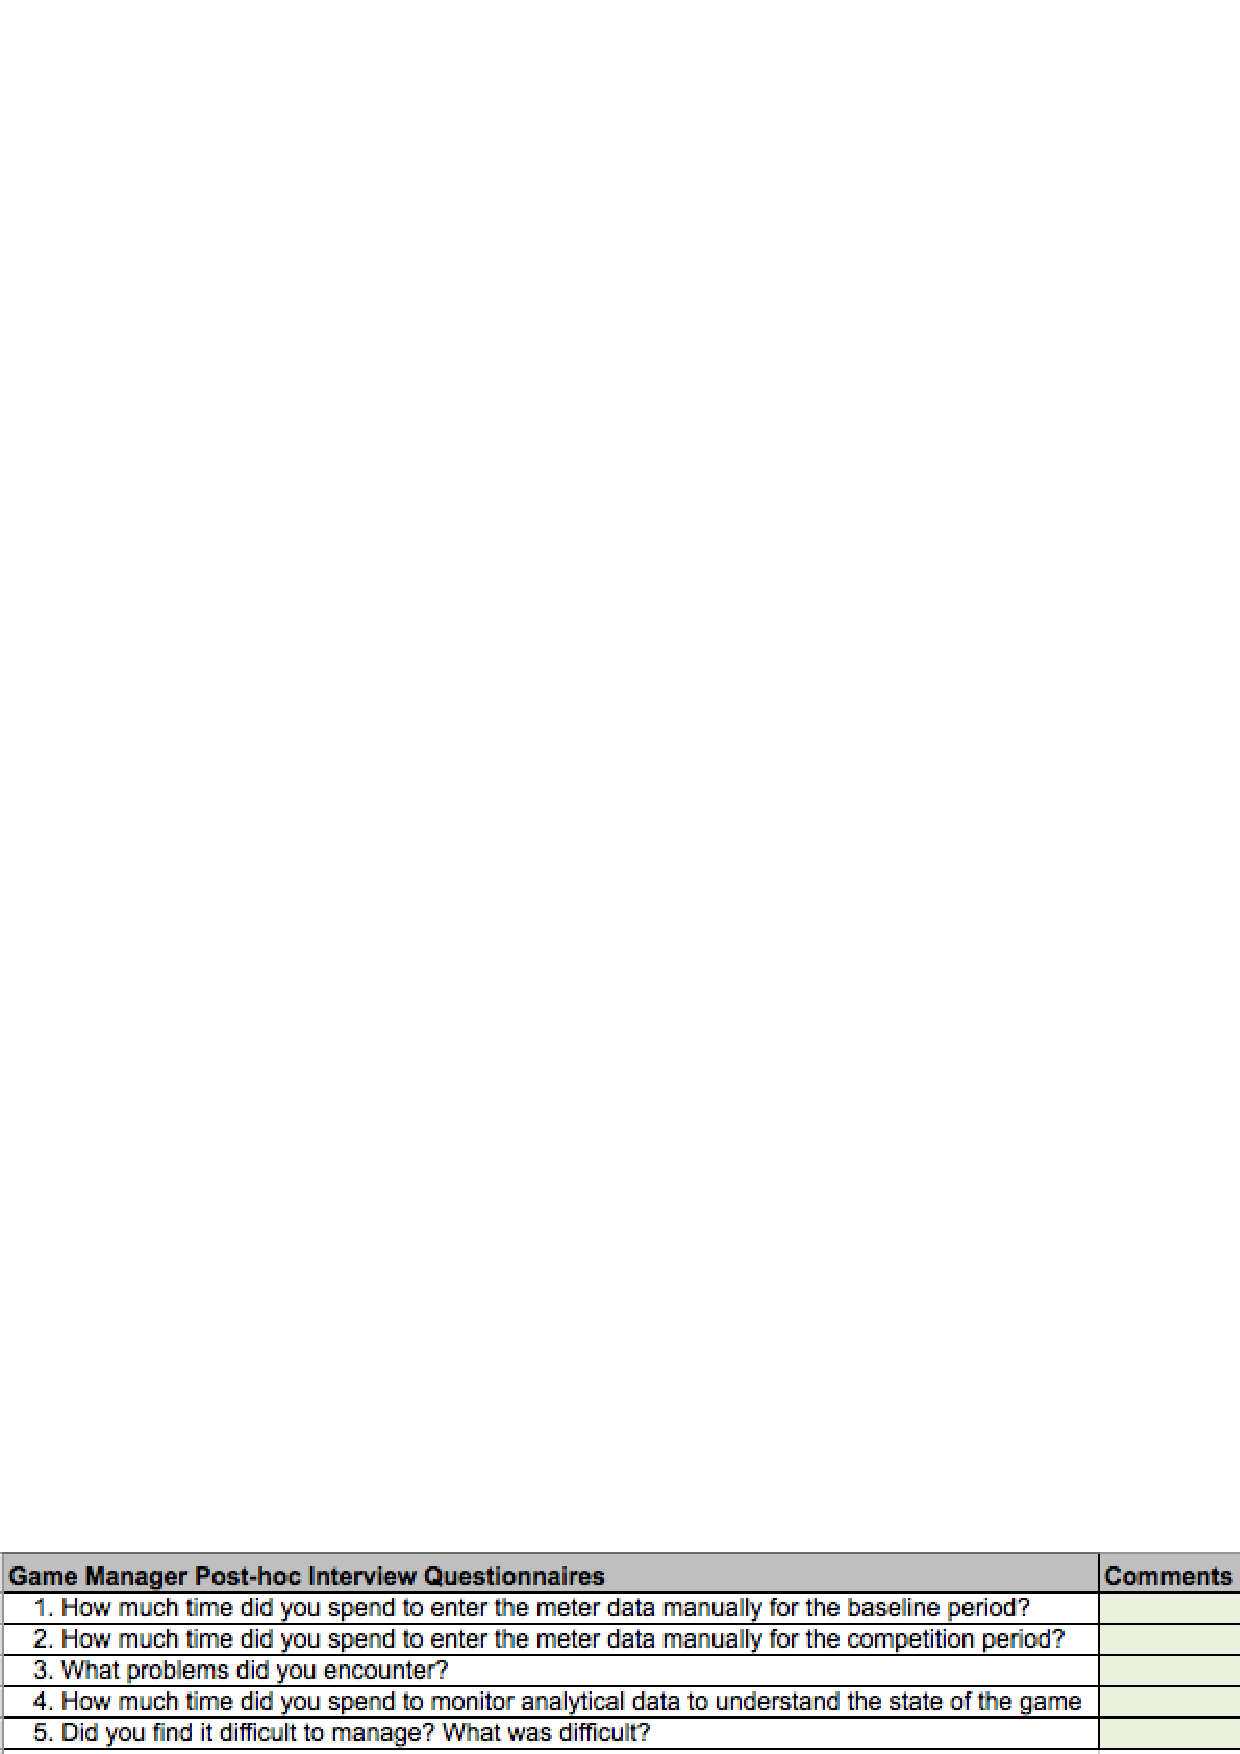
\includegraphics[width=0.9\columnwidth]{manager}
  \caption{Game Manager Assessment}
  \label{table:manager}
\end{table}


\begin{shadebox}
{\bf Action Item:} Review the Game Manager tab in the attached
spreadsheet.  Provide comments for any Game Manager interview questionnaires that
you believe might need to be changed. 
\end{shadebox}

\subsection{Assess Game Developer Stakeholder Experience}

We recommend the post-hoc game developer interview approach for assessing game developer stakeholder experiences. The attached spreadsheet outlines the planned questionnaires for game developer interview, as shown in \autoref{table:developer}.

\begin{table}[ht!]
  \center
  
\includegraphics[width=0.9\columnwidth]{developer}
  \caption{Game Developer Assessment}
  \label{table:developer}
\end{table}


\begin{shadebox}
{\bf Action Item:} Review the Game Developer tab in the attached
spreadsheet.  Provide comments for any Game Developer interview questionnaires that
you believe might need to be changed. 
\end{shadebox}

\section{Step 2: Gather Data}

Once the plan has been finalized, the next step is to carry out the assessment, record the data, obtain log
data, and (if necessary) refine the assessment plan.  The output of this
step is a data repository contains all the assessment data that can be
analyzed in the next step.

\subsection{Carry Out Assessments}

For each stakeholder group, we will complete the tasks outlined in the
assessment plan, gathering the data.

\subsection{Obtain log data}

Certain assessments (such as player engagement) depend upon access to
certain kinds of log data.  We will confer with technical staff as to
how to obtain this data. 

\section{Step 3: Produce Assessment Report}

In this step, we will analyze the data gathered from previous steps,
create an analysis of the strengths and weakness of the framework, 
and produce an action report with our recommendations as to framework improvements.

\subsection{Analyze Data}

Our analysis will include qualitative analysis of questionnaire data
as well as quantitative analysis of log data. For example, for player
assessment, we will calculate the engagement metrics from the game
log; for game designer assessment, we will analyze interaction log
data to find out the completion time for a certain game design tasks.

\subsection{Determine Strength and Weakness}

We will attempt to determine the most important problem areas from our
data and summarize them, as well as the areas where the framework
appears to be most successful.

\subsection{Produce Report with Actionable Steps}

Once the strengths and weaknesses of the framework are identified from
the data analysis, an action report should be produced.  This report
includes the weakness areas that can be improved and actionable steps
on how to improve from each stakeholder's perspective. It also
includes strengths that the framework needs to maintain.

This concludes the SGSEAM assessment.

\section{SGSEAM Assessment Approaches for BuildingOS}
\label{app:sgseam-approaches}

There are usually multiple assessment approaches for each stakeholder.  \autoref{table:approaches} provides 
an overview of the assessment method and the approaches. The appropriate assessment approaches should 
be determined according to the resource available. The approaches for a stakeholder is additive. The more 
approaches applied, the higher confidence of the assessment can be achieved. 

\begin{table}[ht!]
  \centering
  \begin{tabular}{|p{0.175\columnwidth}|p{0.3\columnwidth}|p{0.43\columnwidth}|}
    \hline
    \tabhead{Stakeholder}&
    \tabhead{Assessment goal}&
    \tabhead{Assessment approaches} \\
    \hline
    Player&
    Determine the extent the framework affect and engage players.&
    	Pre-post effectiveness study(\ref{Pre-Post effectiveness study});\newline
	Self-reported usability survey(\ref{Self-reported usability survey});\newline
	Engagement metrics(\ref{Engagement metrics}) \\
    \hline
    System admin&
    Determine strengths and weaknesses in system install and maintenance.&
    	Post-hoc admin interview(\ref{Post-hoc system admin interview});\newline
	In-lab system admin study(\ref{In-lab system admin study}) \\
    \hline
    Game designer&
    Determine strengths and weaknesses in facilitating the game design process.&
    	Post-hoc designer interview(\ref{Post-hoc game designer interview});\newline
	In-lab game design study(\ref{In-lab game design study})\\
    \hline
    Game manager&
    Determine strengths and weaknesses in managing the game.&
    	Post-hoc manager interview(\ref{Post-hoc game manager interview});\newline
	In-lab game management study(\ref{In-lab game management study})\\
    \hline
    Game developer&
    Determine strengths and weaknesses in developing system enhancement.&
    	Post-hoc developer interview(\ref{Post-hoc game developer interview});\newline
	In-lab game development study(\ref{In-lab game development study}) \\
    \hline
  \end{tabular}
  \caption{SGSEAM approaches}
  \label{table:approaches}
\end{table}

The following sections describe in detailed the different approaches for each stakeholder.  Each assessment 
approach describes the goal of the assessment, what data to collect, how to collect the data and how to 
analyze the data to obtain insights about the strengths and weaknesses of the framework from each 
stakeholder's perspective.

\section{Player Assessment}

The goal of player assessment is to determine the effectiveness of the game
framework from player's perspective as well as the usability of the game interface and the engagement level of the game. 
We proposes three approaches for assessing the player's experience with Lucid's framework.

\subsection{Player Assessment Approach: Pre-post Effectiveness Study}
\label{Pre-Post effectiveness study}

One of the goals of the competition is (but not limited to) the reduction of resource such as energy and water consumption. To assess the effectiveness of this goal, we need to determine the metrics that may be measured before and after the competition (pre-post). Lucid BuildingOS and Dashboard calculates the percentage of reduction of energy and water consumption for each participated building, based on the baseline usage of the previous two weeks. We will use this metrics to measure the effect of the competition. The maximum, minimum and average percentage of reduction of all the buildings are calculated to determine the most, the least and average reduction of the resource usage. 

This assessment reveals the extend of effectiveness of the game produced by the framework, regarding to the resource consumption reduction. 
  
\subsection{Player Assessment Approach: Self-reported Usability Survey} 
\label{Self-reported usability survey}

We will conduct a player usability survey at the final week or right after the competition to understand the strengths and weaknesses of the game user interface perceived by players. Minimum of 20 players (the more the better) are randomly selected to participate in this survey. The survey is administrated online via survey monkey or other survey tools. We design the survey questionnaire as shown in \autoref{fig:usability-metrics}.
       
\begin{table}[ht!]
\begin{mybox}
\begin{compactenum}
\item What did you like most about the game?
\item What did you found confusing?
\item What issues did you have while using the game?
\item What was the thing you liked the least about the game?
\item What can we do to improve the game?
\item It was easy to find what I was looking for on the website.  \\
	Strongly disagree  -  Disagree  -  Neutral  -  Agree  -  Strongly agree
\item The website was responsive. \\
	Strongly disagree  -  Disagree  -  Neutral  -  Agree  -  Strongly agree
\item The website provided adequate help in teaching me how to play. \\
	Strongly disagree  -  Disagree  -  Neutral  -  Agree  -  Strongly agree
\item I understood how to play. \\
	Strongly disagree  -  Disagree  -  Neutral  -  Agree  -  Strongly agree
\item this is something my friends should participate in. \\
	Strongly disagree  -  Disagree  -  Neutral  -  Agree  -  Strongly agree
\end{compactenum}
\end{mybox}
\caption{Player self-reported usability survey questionnaires}
\label{fig:usability-metrics}  
\end{table}

Once the survey is created online, the survey administrator will email the selected players with the link and instruction to the online survey. 
After we received all the survey responses, we will code and analyze the response to understand the areas of usability problems in the game interface as well as the areas of strengths.

This assessment reveals the strengths and weaknesses of the framework regarding the usability of the game interface.
 
\subsection{Player Assessment Approach: Engagement Metrics}
\label{Engagement metrics}

This approach calculates the engagement metrics to assess the extent of engagement from players and the impact of the game. The more engaging the game is, the more potential impact could be to the players.

We will first obtain the detailed logs of user interaction with the game. These logging includes http web server logs and user action logs which identify every user click on the web page. Once the log data are available, we will calculate the engagement metrics as described in \autoref{figure:engagement-metrics}. Calculate as many as possible the player engagement metrics. The more metrics obtained, the better understanding of the extent of player engagement.

\begin{table}[ht!]
  \centering
    \begin{tabular}{|p{0.18\columnwidth}|p{0.29\columnwidth}|p{0.32\columnwidth}|}
    \hline
    \tabhead{Metric} &
    \tabhead{Definition} &
    \tabhead{Mesure} \\
    \hline
    participation &
    percentage of players who participated in the game  &
    the level of involvement from players \\
    \hline
    daily player &
    average percentage of players per day &
    the frequency of players interact with the game \\
    \hline
    daily play time &
    average play time of a player per day &
    the frequency of players interact with the game \\
    \hline
    submission &
    average submissions of a player &
    the rate of players' completion of game activities \\
    \hline
    social interaction &
    average social interaction of a player &
    the rate of in-game social interactions between players\\
    \hline
    game error &
    percentage of players who encountered errors &
    the rate of errors encountered by players during the game \\
    \hline
  \end{tabular}
  \caption{Player engagement metrics}
  \label{figure:engagement-metrics}
\end{table}

With the exception of the game error metric, the higher value these metrics are, the higher engagement level the game has. 
Distribution of the above metrics across of the period of the competition also provides insights on 
the extent of engagement in different time of the competition. For example, it may be typical that
the first few days of the competition may have higher number of player and play time metrics because 
of the launch, or due to the announcement of an interesting real-world event. 

This assessment reveals the extent of engagement of the players in the game.

\section{System Admin Assessment}

The goal of system admin assessment is to determine to what extent the 
framework facilitates the system administration tasks from system admin's perspective. SGSEAM 
assesses how much time is required to install and maintain an instance of a serious game using the 
framework and the problems encountered  during the system admin process.

We consider the tasks of system admin interacting with Lucid's framework are:
\begin{compactenum}
    \item install the software
    \item configure smart meter connectivity
    \item backup data
    \item monitor performance
    \item scaling the system
    \item patching
\end{compactenum}

We propose the post-hoc system admin interview approach to assess the system admin's experience for Lucid's framework.

\subsection{System Admin Assessment Approach: Post-loc System Admin Interview}
\label{Post-hoc system admin interview}

Once we identify the contact information of the system admins, the interview will be administrated by using an online questionnaire form followed by an optional phone interview if needed. We design the interview with the following questionnaire that is tailored to the specific tasks of the system admins of Lucid's framework:

\begin{table}[ht!]
\begin{mybox}
\begin{compactenum}
\item How much time did you spend to install the system and the dependencies?
\item How much time did you spend to configure the meters?
\item How much time did you spend to maintain the system such as backup, patching, monitoring?
\item Did you need to scale the system? if Yes, how much time did you spend?
\item What problems did you encounter?
\item Did you find it difficult to admin the system? What was difficult?
\item Do you agree for us to call you for a short phone interview if we have more questions regarding your experience with the system?
\end{compactenum}
\end{mybox}
\caption{System admin interview questionnaires}
\label{fig:system-admin-interview}  
\end{table}

Once we receive the responses from the system admin, we will code (categorize) the time and problems encountered to find out what are the problem areas if there is any. if we need further explanation to the response, we will administrate a quick phone interview to address the specific response. 

These assessment reveals the strengths, weaknesses and the areas of improvement regarding the system admin process for the framework.

\subsection{System admin assessment approach: In-lab system admin study (Not Recommended for Lucid)}
\label{In-lab system admin study}

This approach assesses the system admin's experience using the in-lab experimental study. First identify a group 
of participants who have some levels of system administration experience. Second, provide instructions on 
each installation steps, ask the participants to install the system according to the instructions, and ask them to record 
the time spent and problems encountered as they complete each step.

Once the experiment data is collected, categorize the reported problems and correlated with the reported time data 
to identify the areas of strength (less time spent) and weakness (more time spent and problems or difficulties). 

Due to the cost of in-lab assessment, this approach is not recommended to Lucid BuildingOS assessment.

\section{Game Designer Assessment}

The goal of SGSEAM game designer assessment is to determine the strengths and weaknesses of the framework 
regarding to the game design process. SGSEAM 
assesses how much time is required to design an instance of a serious game using the framework and the problems encountered during the design process.

We consider the tasks of game designer interacting with Lucid's framework are:
\begin{compactenum}
    \item decide competition period
    \item set up building occupancy, manual or automated meters
    \item decide baseline period
    \item monitor competition status during the competition
\end{compactenum}

We propose the post-hoc game designer interview approach to assess the game designer's experience.

\subsection{Game Designer Assessment Approach: Post-hoc Game Designer Interview}
\label{Post-hoc game designer interview}

 The interview is administrated by using an online questionnaire form followed by an optional phone interview if needed. We will interview several game designers of different competitions. The more data we collect, the more insights we get. The interview is designed with the following questionnaire that is tailored to the specific tasks of the game designers of Lucid's framework:

\begin{table}[ht!]
\begin{mybox}
\begin{compactenum}
\item How much time did you spend to set up the buildings including meters?
\item How much time did you spend to setup the competition (competition periods, baseline period, participants)?
\item How much time did you spend to setup the homepage by deciding which widgets to include?
\item How much time did you spend to monitor analytical data to understand the state of the game
\item What problems did you encounter?
\item Did you find it difficult to use the interface? What was difficult?
\item Do you agree for us to call you for a short phone interview if we have more questions regarding your experience with the system?
\end{compactenum}
\end{mybox}
\caption{Game designer interview questionnaires}
\label{fig:game-designer-interview}  
\end{table}

After the interview, code and categorize the reported time and problems to identify the strengths and weaknesses. In addition, if possible, collect the system log data related to the game designing tasks, analyze the logs to find out the time spent and error encountered during the game designing tasks. Use the log data to verify the findings from the interview data.

These assessment reveals the strengths, weaknesses and the areas of improvement regarding the game design process for the framework.

\subsection{Game designer assessment approach: In-lab game design study (Not Recommended for Lucid)}
\label{In-lab game design study}

This approach assesses the game designer experience using the in-lab experimental study.  First identify a group 
of participants who are somewhat familiar with the subject domain of the game. Second, provide instructions on 
each designing steps, ask the participants to design the game according to the instructions, ask them to record 
the time spent and problems encountered as they complete each step.

Once the experiment data is collected, categorize the reported problems and correlated with the reported time data 
to identify the areas of strength (less time spent) and weakness (more time spent and problems or difficulties). 

Due to the cost of in-lab assessment, this approach is not recommended to Lucid BuildingOS assessment.

\section{Game Manager Assessment}

The goal of SGSEAM game manager assessment is to determine the strengths and weakness of the framework 
regarding to the game management process. Similar to the assessment of the game designer, SGSEAM assesses 
how much time it is required to manage an instance of a serious game using the framework
and the problems encountered during the managing process.

We consider the tasks of game manager interacting with Lucid's framework are:
\begin{compactenum}
    \item input data manually
    \item manage events, marketing, handing out prizes
    \item monitor competition status
\end{compactenum}

we propose the post-hoc game manager interview approach for assessing game manager's experience.
    
\subsection{Game Manager Assessment Approach: Post-hoc Game Manager Interview}
\label{Post-hoc game manager interview}

 The interview is administrated by using an online questionnaire form followed by an optional phone interview if needed. We will interview several game managers of different competitions. The more data we collect, the more insights we get.  The interview is designed with the following questionnaire that is tailored to the specific tasks of the game managers of Lucid's framework:

\begin{table}[ht!]
\begin{mybox}
\begin{compactenum}
\item How much time did you spend to enter the meter data manually for the baseline period?
\item How much time did you spend to enter the meter data manually for the competition period?    
\item What problems did you encounter?
\item How much time did you spend to monitor analytical data to understand the state of the game
\item Did you find it difficult to manage? What was difficult?
\end{compactenum}
\end{mybox}
\caption{Game manager interview questionnaires}
\label{fig:game-manager-interview}  
\end{table}

After the interview, code and categorize the reported time and problems to identify the strengths and weaknesses in the game managing process. In addition, if possible, collect the system log data related to the game managing tasks, analyze the logs to find out the time spent and error encountered during the game managing tasks. Use the log data to verify the findings from the interview data.

These assessment reveals the strengths, weaknesses and the areas of improvement regarding the game managing process for the framework.

\subsection{Game manager assessment approach: In-lab game management study (Not Recommended for Lucid)}
\label{In-lab game management study}

This approach assess the game manager's experience using the in-lab game management study.  First identify a group 
of participants who are somewhat familiar with the subject domain of the game. Second, provide instructions on 
each managing tasks, ask the participants to complete the tasks following the instructions, ask them to record 
the time spent and problems encountered as they complete each task.

Once the experiment data is collected, categorize the reported problems and correlated with the reported time data 
to identify the areas of strength (less time spent) and weakness (more time spent and problems or difficulties). 

Due to the cost of in-lab assessment, this approach is not recommended to Lucid BuildingOS assessment.

\section{Game Developer Assessment}

To investigate how easy it is to understand, extend, and debug a serious game framework from a developer's 
perspective, SGSEAM assesses how much time it takes to develop an
enhancement to the game framework, and how many errors are encountered
during the development process.

We consider the tasks of game manager interacting with Lucid's framework are:

\begin{compactenum}
  \item use API to get data in and/or out of the system
  \item customize the interface
  \item extend the system to support new meters
  \item enhancement
\end{compactenum}

We propose the post-hoc game developer interview approach to assess the game developer's experience.
    
\subsection{Game Developer Assessment Approach: Post-hoc Game Developer Interview}
\label{Post-hoc game developer interview}

BuildingOS and Dashboard have APIs for developing apps to tie into the framework. We will use the API to develop an extension or customization of the system. Here are the development tasks we proposed to perform using Lucid's API to extend the framework:
\begin{compactenum}
  \item create a new widget to be available in the home page.
  \item support the automated energy data collection from a new type of meter.
\end{compactenum}

We will ask the identified game developers to perform the above development tasks using Lucid's framework. The developer could be Lucid internal developers or some one outside of Lucid.  After the development tasks are completed, we will interview the developers to assess his experience for these development tasks. The interview is designed with the questionnaire outlined in \autoref{fig:game-developer-interview}.

\begin{table}[ht!]
\begin{mybox}
\begin{compactenum}
\item How much time did you spend to implement the creation of a new widget?
\item How much time did you spend to implement adding a new type of meter?
\item What problem(s) did you encounter?
\item Did you find it difficult to understand, extend and debug the system? What was difficult?
\end{compactenum}
\end{mybox}
\caption{Game developer interview questionnaires}
\label{fig:game-developer-interview}  
\end{table}

Once the interview data is collected, categorize the reported problems and correlated with the reported time data to identify the areas of strength (less time spent) and weakness (more time spent and problems or difficulties) in the process of development. 

These assessment reveals the strengths, weaknesses and the areas of improvement regarding the game development process for the framework.

\subsection{Game developer assessment approach: In-lab game development study (Not Recommended for Lucid)}
\label{In-lab game development study}

This approach assess the game developer's experience using the in-lab game development study.  
First identify the general development skills that the framework requires, such as the programming language. 
Second, identify a group of participants who have some levels of the required development skills. Third, provide 
requirement specification or instructions on how to develop a new enhancement to the system, ask the 
participants to complete the task, record the time spent and problems encountered as they works on the task.

Once the experiment data is collected, categorize the reported problems and correlated with the reported time data 
to identify the areas of strength (less time spent) and weakness (more time spent and problems or difficulties). 

Due to the cost of in-lab assessment, this approach is not recommended to Lucid BuildingOS assessment.
